\documentclass{beamer}
\usepackage{tcolorbox}
\usepackage{graphicx}
\usepackage{amsmath}
\usepackage[labelformat=empty]{caption}
\usepackage{subcaption}

\usepackage{hyperref}
\hypersetup{
    colorlinks=true,
    linkcolor=blue,
    filecolor=magenta,      
    urlcolor=cyan,
}

\usepackage{tikz}
\def\checkmark{\tikz\fill[scale=0.4](0,.35) -- (.25,0) -- (1,.7) -- (.25,.15) -- cycle;} 


%\beamerdefaultoverlayspecification{<+->}
\newcommand{\data}{\mathcal{D}}

\DeclareMathOperator*{\argmin}{arg\,min}

\newcommand\Item[1][]{%
	\ifx\relax#1\relax  \item \else \item[#1] \fi
	\abovedisplayskip=0pt\abovedisplayshortskip=0pt~\vspace*{-\baselineskip}}
	


\usetheme{metropolis}           % Use metropolis theme


\title{Ridge Regression}
\date{\today}
\author{Nipun Batra}
\institute{IIT Gandhinagar}
\begin{document}
  \maketitle
  
\begin{frame}{Introduction}
\vspace{0.9cm}
To prevent over fitting we place penalties on large $\theta_i$
\pause
\vspace{-0.4cm}
\begin{figure}
        \begin{subfigure}[b]{0.5\textwidth}
                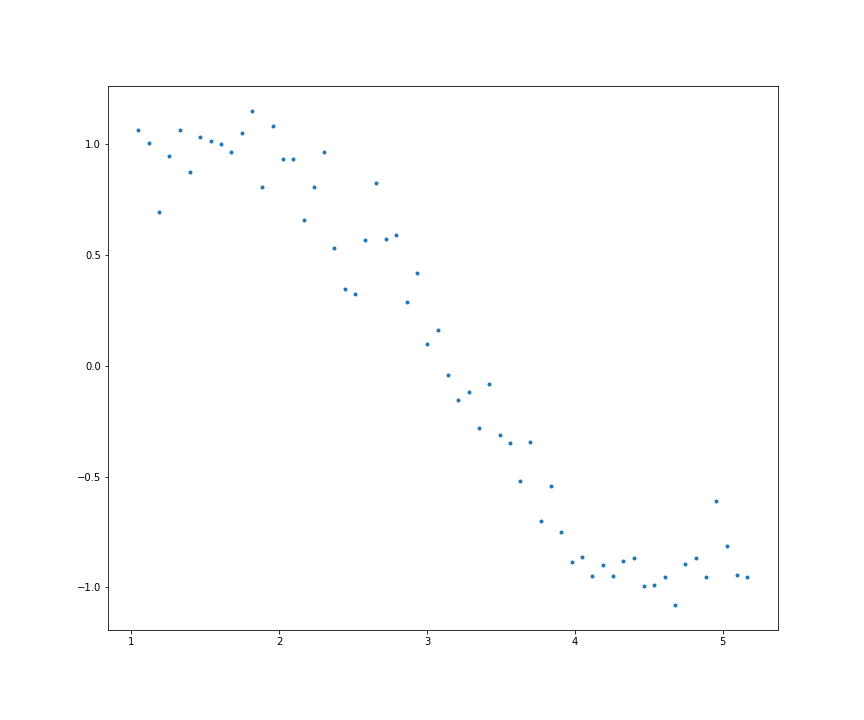
\includegraphics[width=\linewidth]{ridge/lin_1.png}
                \caption{Base Data Set}
        \end{subfigure}%
        \begin{subfigure}[b]{0.5\textwidth}
                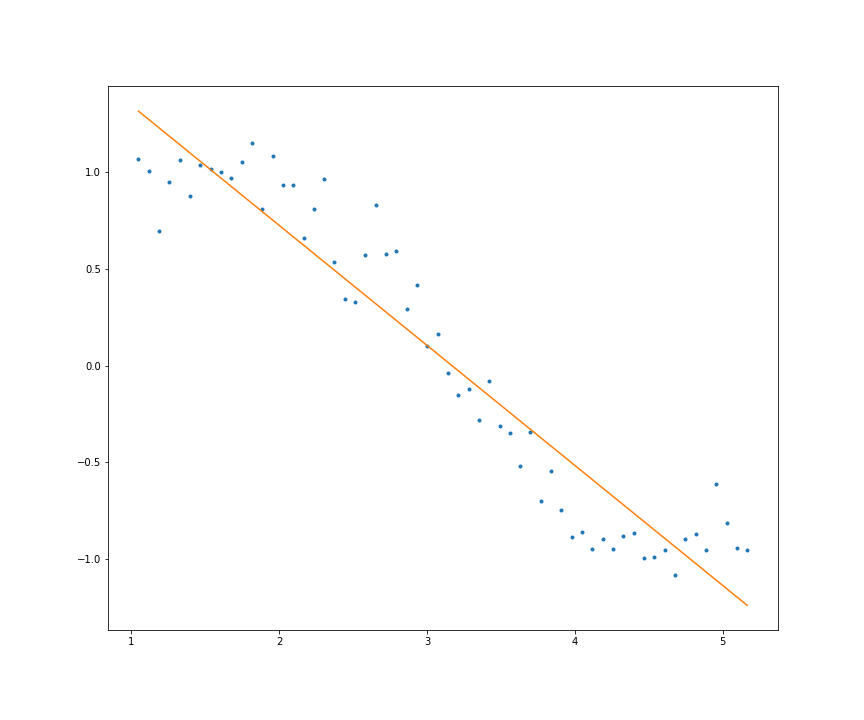
\includegraphics[width=\linewidth]{ridge/lin_plot_1.png}
                \caption{Degree 1 (Coeff. = $-0.62$)}
        \end{subfigure}%
        \caption{An example of over fitting}
\end{figure}
\end{frame}  

\begin{frame}{Introduction}
\vspace{0.9cm}
To prevent over fitting we place penalties on large $\theta_i$
\vspace{-0.4cm}
\begin{figure}
        \begin{subfigure}[b]{0.5\textwidth}
                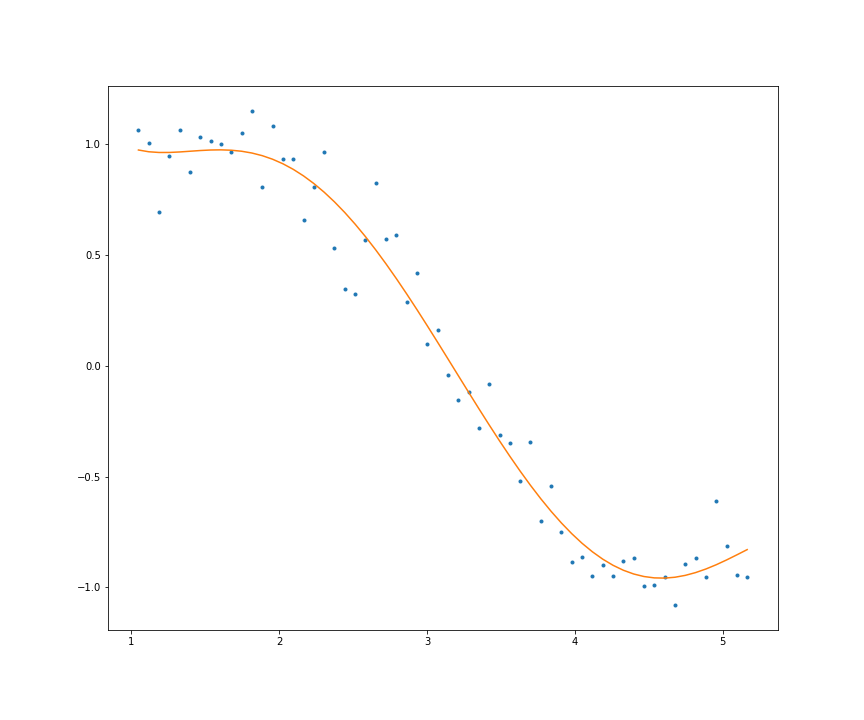
\includegraphics[width=\linewidth]{ridge/lin_plot_5.png}
                \caption{Degree 5 (Coeff. = $-5.12$)}
        \end{subfigure}%
        \begin{subfigure}[b]{0.5\textwidth}
                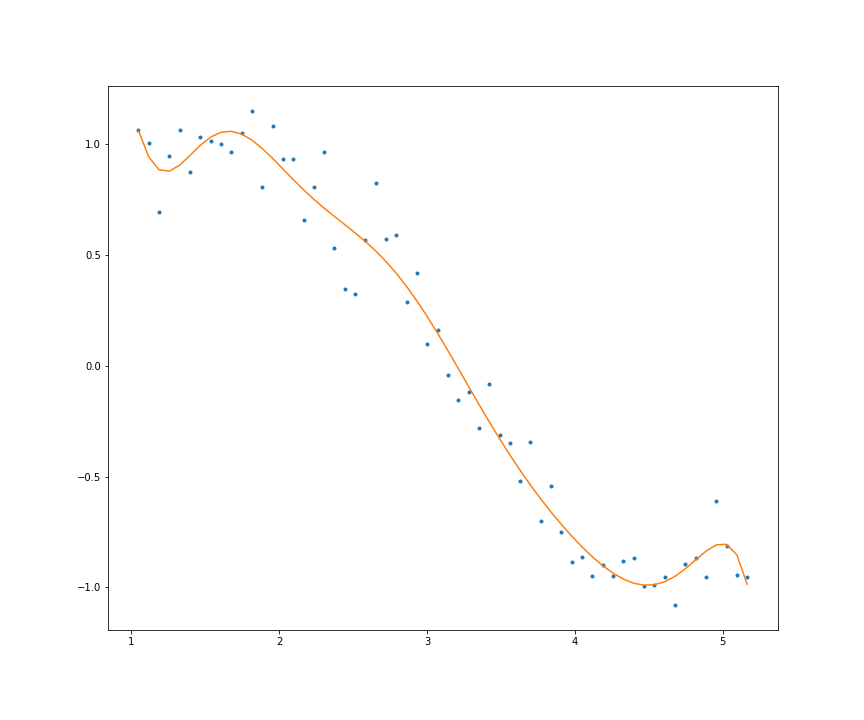
\includegraphics[width=\linewidth]{ridge/lin_plot_12.png}
                \caption{Degree 12 (Coeff. = $6007.88$)}
        \end{subfigure}%
        \caption{An example of over fitting}
\end{figure}
\end{frame}  
  
\begin{frame}{Introduction}
\vspace{0.4cm}
To prevent over fitting we place penalties on large $\theta_i$
 \\ \bigskip
\begin{tcolorbox}{Objective}
\begin{align*}
\text{Minimize } & \left(y-x\theta\right)^T\left(y-x\theta\right) \\
\text{s.t. } & \theta ^T\theta \leq S
\end{align*}
\end{tcolorbox}
\pause
This is equivalent to \vspace{-0.4cm}
$$
\text{Minimize } \left(y-x\theta\right)^T\left(y-x\theta\right) + \delta ^2\theta ^T\theta
$$
\end{frame}  

\begin{frame}{KKT Conditions}
To implement this we use KKT Conditions
\pause
\begin{align*}
\text{Minimize } & \left(y-x\theta\right)^T\left(y-x\theta\right) \\
\text{s.t. } & \theta ^T\theta \leq S \\
L\left(\theta, \mu \right) =& \left(y-x\theta\right)^T\left(y-x\theta\right) + \mu\left(\theta^T\theta - S\right)
\end{align*}
where, $\mu \geq 0$ \bigskip

\pause
\begin{columns}
\begin{column}{0.4\textwidth}
If $\mu = 0$ \\
There is no regularization \\
No effect on constraint
\end{column}
\pause
\begin{column}{0.4\textwidth}
If $\mu\neq 0$ \\
$\implies \theta^T\theta - S = 0$ 
\end{column}
\end{columns}
\end{frame}

\begin{frame}{Effect of $\mu$}
\begin{figure}
        \begin{subfigure}[b]{0.5\textwidth}
                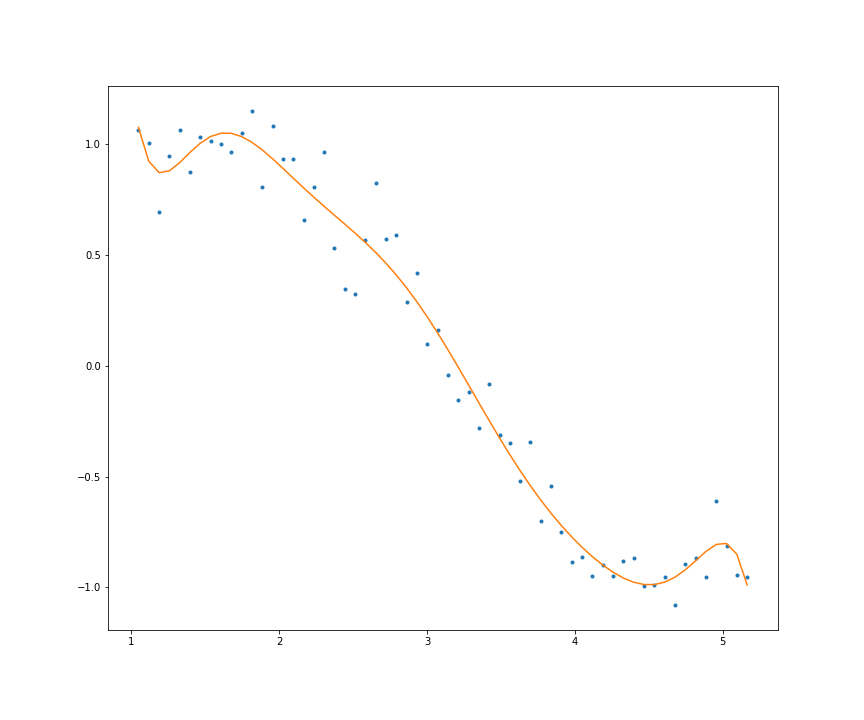
\includegraphics[width=\linewidth]{ridge/rid_plot_15.png}
                \caption{$\mu = 1e-15$}
        \end{subfigure}%
        \begin{subfigure}[b]{0.5\textwidth}
                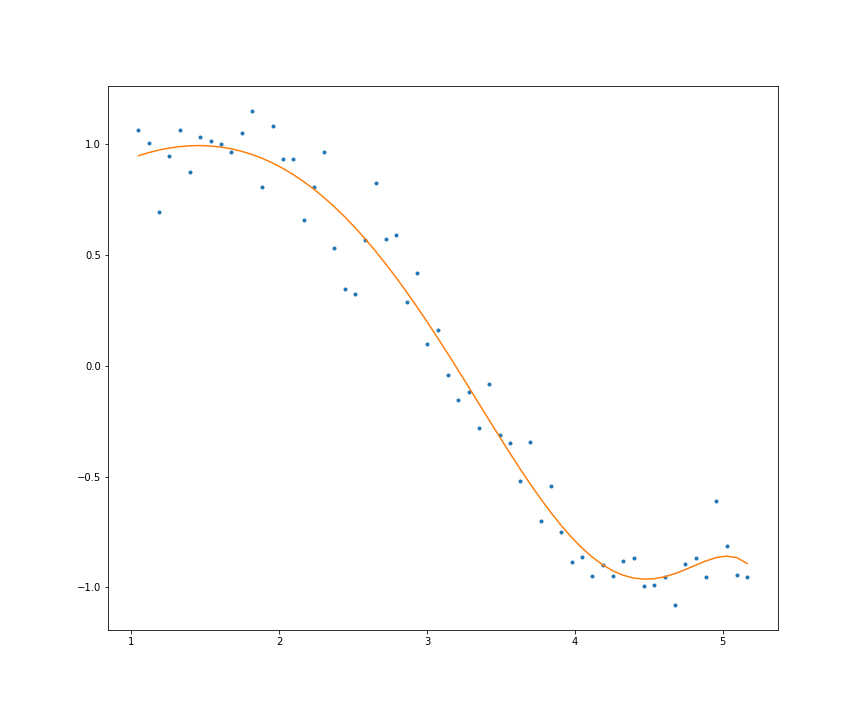
\includegraphics[width=\linewidth]{ridge/rid_plot_4.png}
                \caption{$\mu = 1e-4$}
        \end{subfigure}%
\end{figure}
\end{frame} 

\begin{frame}{Effect of $\mu$}
\begin{figure}
        \begin{subfigure}[b]{0.5\textwidth}
                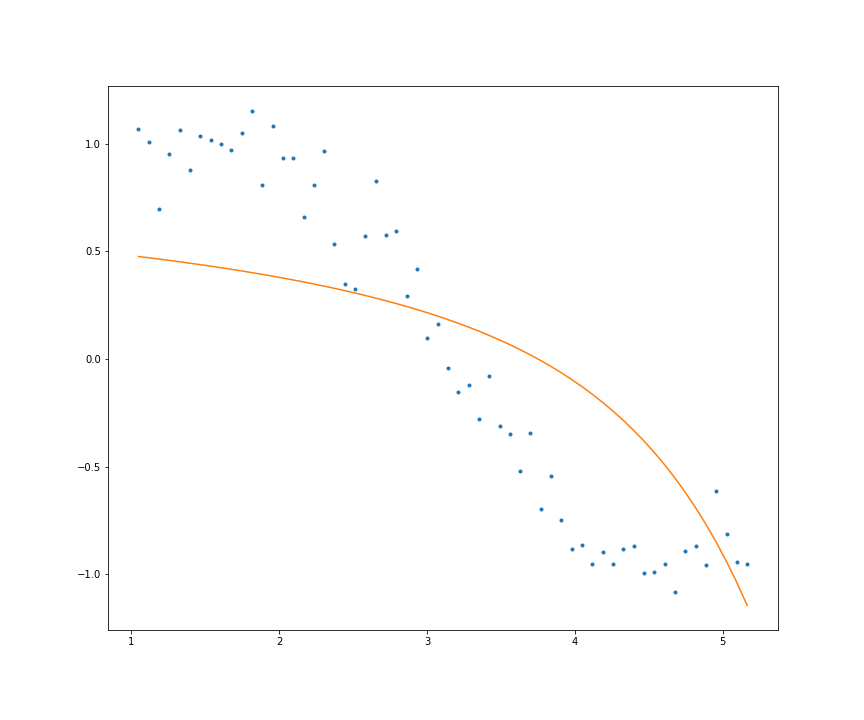
\includegraphics[width=\linewidth]{ridge/rid_plot_5.png}
                \caption{$\mu = 5$}
        \end{subfigure}%
        \begin{subfigure}[b]{0.5\textwidth}
                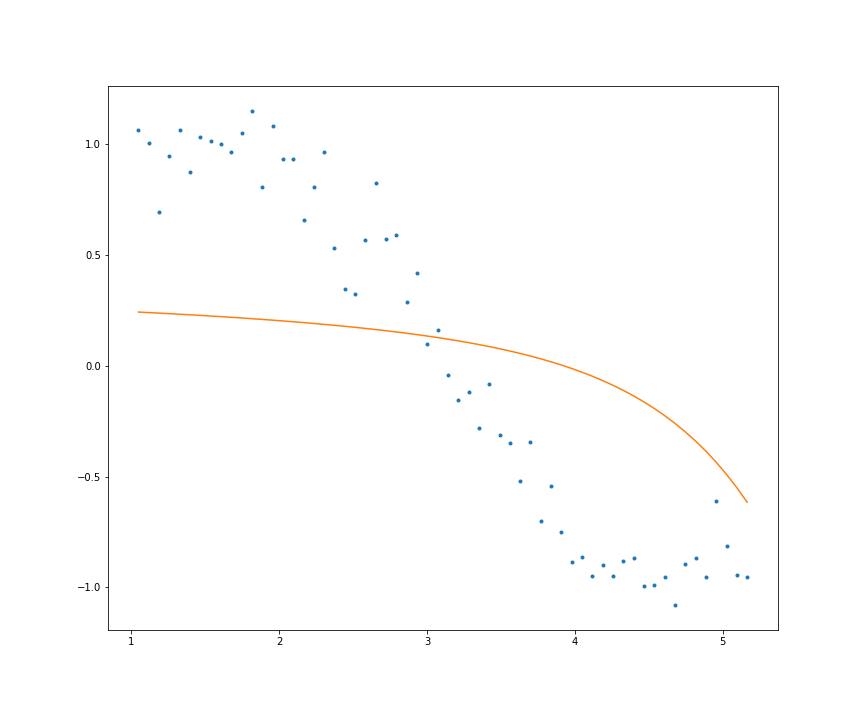
\includegraphics[width=\linewidth]{ridge/rid_plot_9.png}
                \caption{$\mu = 20$}
        \end{subfigure}%
\end{figure}
\end{frame}

\begin{frame}{Effect of $\mu$}
\begin{figure}
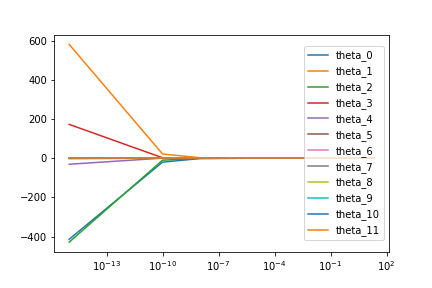
\includegraphics[width=\linewidth]{ridge/rid_reg.png}
\vspace{-0.8cm}
\caption{Effect of $\mu$ on the magnitude of the parameters}
\end{figure}
\end{frame}

\begin{frame}{Analytical Method}
\begin{tcolorbox}{Ridge Objective}
\vspace{-0.4cm}
$$
\min_\theta \left(y-x\theta\right)^T\left(y-x\theta\right)\delta^2\theta^T\theta
$$
\end{tcolorbox}
\begin{align*}
\frac{\partial L\left(\theta, \mu\right)}{\partial \theta} &= 0 \\ 
\frac{\partial}{\partial \theta}\left\lbrace y^Ty - 2y^Tx\theta + \theta^Tx^Tx\theta \right\rbrace + \frac{\partial}{\partial \theta} \delta^2\theta^T\theta &= 0 \\
\implies -x^Ty + \left(x^Tx + \delta^2I\right)\theta &= 0 \\
\implies \theta^* &= \left(x^Tx + \delta^2I\right)^{-1}x^Ty
\end{align*}
\end{frame}

\begin{frame}{Bias/Variance}
\begin{columns}
\begin{column}{0.4\textwidth}
\begin{figure}
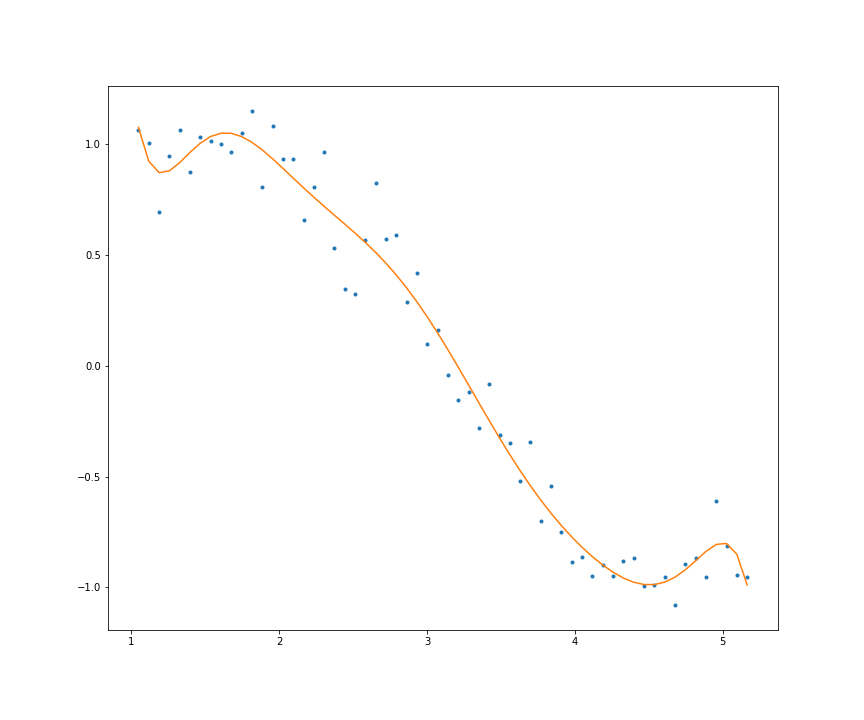
\includegraphics[width=\linewidth]{ridge/rid_plot_15.png}
\end{figure}
Fit High Order Polynomial \\
$\implies$ high variance \\
$\implies \, \delta^2 \rightarrow 0$
\end{column}
\begin{column}{0.4\textwidth}
\begin{figure}
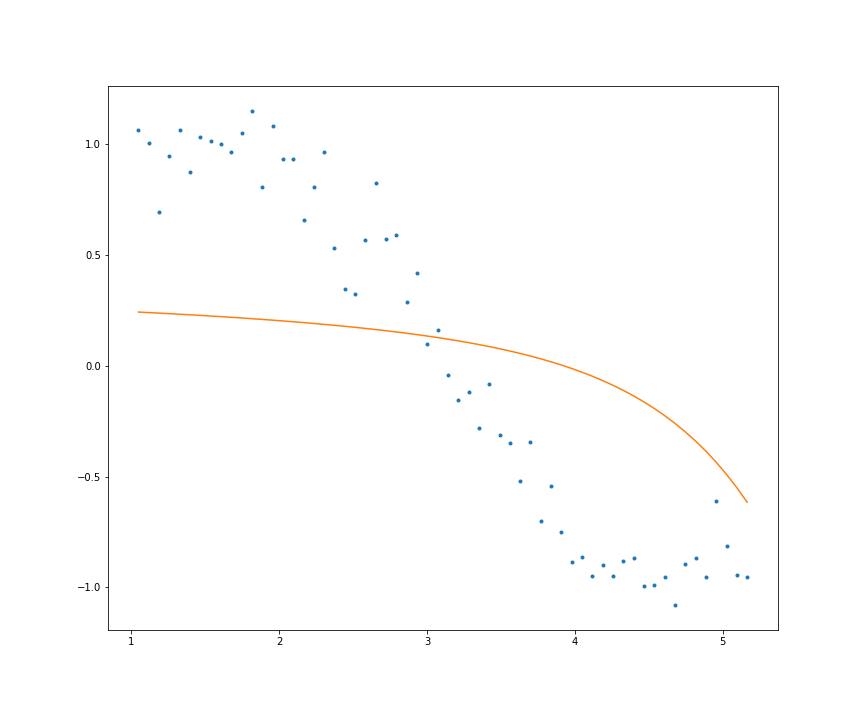
\includegraphics[width=\linewidth]{ridge/rid_plot_9.png}
\end{figure}
Fit High Order Polynomial \\
$\implies$ low variance \\
$\implies \, \delta^2 \rightarrow \infty$
\end{column}
\end{columns}
\end{frame}

\begin{frame}{Example}
\vspace{0.4cm}
\textbf{Q.)} Solve Regularized ($\delta^2 = 2$) and Unregularized.
\vspace{-0.6cm}
\begin{figure}
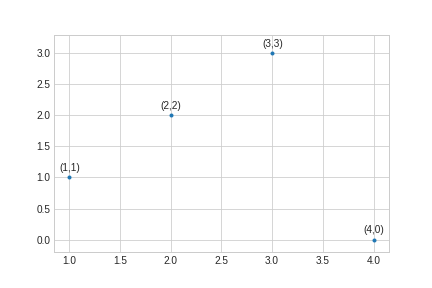
\includegraphics[width=\linewidth]{ridge/ques_1.png}
\end{figure}
\end{frame}

\begin{frame}{Example}
\vspace{0.4cm}
For Unregularized, $\hat{y} = 2-0.2x$
\vspace{-0.6cm}
\begin{figure}
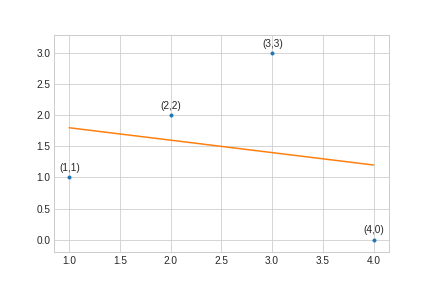
\includegraphics[width=\linewidth]{ridge/ques_2.png}
\end{figure}
\end{frame}

\begin{frame}{Example}
\vspace{0.4cm}
For Regularized, $\hat{y} = 0.5+0.4x$
\vspace{-0.6cm}
\begin{figure}
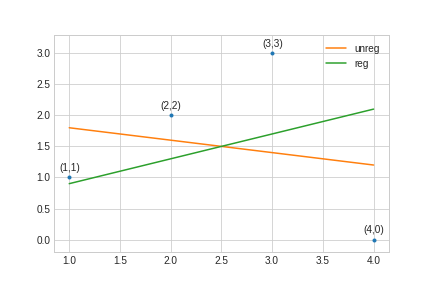
\includegraphics[width=\linewidth]{ridge/ques_3.png}
\end{figure}
\end{frame}

\begin{frame}{Extension of the analytical model}
For ridge with no penalty on $\theta_0$
$$
\hat{\theta} = \left(x^Tx+\delta^2I^*\right)^{-1}x^Ty
$$
where, $$I = \begin{bmatrix}
    0 & 0 & 0 & \dots  & 0 \\
    0 & 1& 0 & \dots  & 0\\
    \vdots & \vdots & \vdots & \ddots & \vdots \\
    0 & 0 & 0 & \dots  & 1
\end{bmatrix}$$
\end{frame}

\end{document}